\pdfminorversion=4
\PassOptionsToPackage{x11names}{xcolor}
\documentclass[aspectratio=169]{beamer}
%\documentclass[handout]{beamer}
%\usepackage{handoutWithNotes}
%\pgfpagesuselayout{4 on 1 with notes}[a4paper, border shrink=5mm]
%% Method from https://github.com/gdiepen/latexbeamer-handoutWithNotes
\usepackage{amsmath}
\usepackage{subcaption}
\usepackage{appendixnumberbeamer}
\usepackage{animate}
\usepackage{grffile}
\usepackage[utf8]{inputenc}
\usepackage{minted}
%\usepackage[hang,flushmargin]{footmisc}

\usepackage{tikz}
\usetikzlibrary{shapes.geometric, arrows, positioning}

\usepackage[style=authortitle,backend=biber]{biblatex}
\addbibresource{refs.bib}

\usetheme{Sheffield}
\useinnertheme{SheffieldCBM}

\addbibresource{library.bib}

\newsavebox{\foobox}
\newcommand{\slantbox}[2][0]{\mbox{%
        \sbox{\foobox}{#2}%
        \hskip\wd\foobox
        \pdfsave
        \pdfsetmatrix{1 0 #1 1}%
        \llap{\usebox{\foobox}}%
        \pdfrestore
}}
\newcommand\unslant[2][-.25]{\slantbox[#1]{$#2$}}

%  \item specially for beamer
\renewcommand{\footnotesize}{\scriptsize}
\renewcommand{\vec}{\mathbf}

\tikzset{
    userblock/.style={
    rectangle,
    rounded corners,
    minimum width=3cm,
    minimum height=1cm,
    align = center,
    text=sgreydark,
    draw=shefblue,
    line width = 1pt,
  },
  flowblock/.style={
    rectangle,
    rounded corners,
    minimum width=2.4cm,
    minimum height=1cm,
    align = center,
    anchor = center,
    text=sgreydark,
    draw=sgreylight,
    line width = 1pt,
  },
  question/.style={
  text=shefblue
  },
  arrow/.style={
    line width = 1.5pt,
    ->,
    > = stealth,
    draw=shefblue,
    rounded corners
    },
  dashdouble/.style={
    line width = 1.5pt,
    <->,
    > = stealth,
    draw=shefblue!70,
    },
  bentarrow/.style={
    line width = 1.5pt,
    ->,
    > = stealth,
    draw=shefblue!70,
    bend left=20,
    },
}

\newenvironment<>{varblock}[2][.9\textwidth]{%
  \setlength{\textwidth}{#1}
  \begin{actionenv}#3%
    \def\insertblocktitle{#2}%
    \par%
    \usebeamertemplate{block begin}%
}{%
  \par%
    \usebeamertemplate{block end}%
  \end{actionenv}%
}

\begin{document}

\title{Here there be dragons}
\subtitle{The HPC Code Development Journey}
\author[phil.tooley@sheffield.ac.uk]{Phil Tooley\\University of Sheffield}
\date[HPC@Sheffield 2019/04/08]{\\8 April 2019}


\begin{frame}
\maketitle
\end{frame}

\begin{frame}
  \centering
  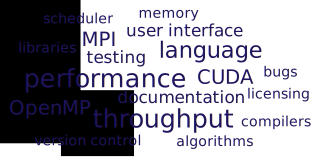
\includegraphics[width=0.8\textwidth]{confusioncloud}
\end{frame}

\begin{frame}
  \centering
  
\includegraphics[width=0.8\textwidth]{georgeanddragon}
\end{frame}

\begin{frame}
  \frametitle{What makes an application HPC?}
  \begin{block}{Anything that your laptop can't do on its own...}
    \begin{itemize}
      \item More compute power
      \item More memory
      \item Specialist hardware
      \item Large dataset storage
      \item Better visualisation
      \item etc...
    \end{itemize}
  \end{block}
\end{frame}

\begin{frame}
  \frametitle{A real world example --- image registration}
  \centering
  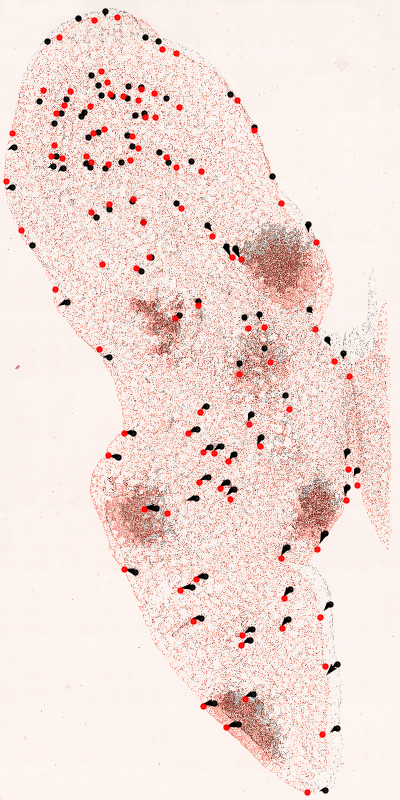
\includegraphics[angle=-90,width=0.7\textwidth]{mapped_annotations}
\end{frame}

\begin{frame}
  \frametitle{How do I write code for an HPC?}
  \begin{block}{Work out what your code needs:}
    \alt<2-3>{
      \alt<3>{
        \begin{block}{GPU Accelerator}
          \begin{itemize}
            \item Code fits in a single node's memory, but needs to be faster
            \item Use 1000s of parallel threads for computation
            \item Needs large, parallel problems for efficient use of hardware
          \end{itemize}
        \end{block}
        \invisible<1-3>{
          \begin{block}{Ghost block}
            \begin{itemize}
              \item ``WOOOO...
              \item ...OOOOO....
              \item ...OOH''
            \end{itemize}
          \end{block}
        }
      }{
        \begin{block}{Shared Memory - Multiple cores on one node}
          \begin{itemize}
            \item Code fits in a single node's memory, but needs to be faster
            \item Parallel algorithms for ``bottlenecks'' in the code
            \item Can often be added to existing serial code
          \end{itemize}
        \end{block}
        \begin{block}{Message Passing - Multiple cores on multiple nodes}
          \begin{itemize}
            \item Need multiple nodes to fit problem in memory
            \item Parallelise data structures and algorithms
            \item Serial code usually needs a complete rewrite
          \end{itemize}
        \end{block}
      }
    }{
      \begin{block}{Large Memory - A bigger node than your laptop}
        \begin{itemize}
          \item Code is fast enough, but need more memory
          \item No changes to ``laptop code''
          \item Use HPC large memory nodes for larger datasets
        \end{itemize}
      \end{block}
      \begin{block}{High Throughput - Run many jobs at once}
        \begin{itemize}
          \item Code is fast enough, but need to run lots
          \item No changes to ``laptop code''
          \item Use HPC to run many jobs in parallel
        \end{itemize}
      \end{block}
    }
  \end{block}
\end{frame}

\begin{frame}
  \frametitle{You can use parallel libraries to help}
  \begin{block}{Low level parallel libraries}
    \begin{itemize}
      \item OpenMP - Shared memory helpers for C/C++/Fortran
      \item MPI - MPI standard implemented by many vendors, available for many languages
      \item CUDA - Run many parallel threads on Nvidia GPUs
      \item OpenACC - OpenMP-like primitives for GPU/Intel MIC offload
      \item Intel TBB - threading building blocks for parallel applications
    \end{itemize}
  \end{block}
  \alert{No maths in these libraries. Just tools to help you write parallel code.}
\end{frame}

\begin{frame}
  \frametitle{But don't reinvent the wheel}
  \begin{block}{Lots of higher level libraries available}
    \begin{itemize}
      \item General high performance math - GSL, MKL, NAG
      \item Linear Algebra - LaPACK, BLAS, Intel MKL
      \item ODE/PDE solvers - PETSc, PVODE, FEniCS
      \item Scientific frameworks - PETSc, Trilinos
      \item Cluster computing - Dask, Hadoop, Spark
      \item Domain specific frameworks - Tensorflow, OpenFOAM, MFEM
    \end{itemize}
  \end{block}
\end{frame}

\begin{frame}
  \frametitle{Managing dependencies}
  \begin{columns}
    \column{0.7\textwidth}
    \begin{block}{Use a dependency manager}
      \begin{itemize}
	\item Give manager a list of required packages and versions
	\item Dependency manager coordinates installation
	\item Loaded using modules just like system provided software
	\item Install multiple versions of a library side-by-side
      \end{itemize}
    \end{block}
    \begin{block}{Easier installation and reproducibility}
      \begin{itemize}
        \item Easier installation for users
        \item Reproducible environment across platforms
        \item Easy testing of dependency versions
      \end{itemize}
    \end{block}
  %
    \column{0.3\textwidth}
    
\includegraphics[width=0.95\textwidth]{easybuild_logo_alpha}
    \vspace{1em}
    
\includegraphics[width=0.95\textwidth]{spack-logo-blue-text}
  \end{columns}
\end{frame}

\begin{frame}
  \frametitle{Writing pFIRE}
  \begin{block}{pFIRE - Image Registration Code}
    \begin{itemize}
      \item Computationally intensive linear algebra
      \item Must scale to very large 3D images --- need lots of memory!
      \item MPI is the best choice -- look for an MPI linear algebra library
    \end{itemize}
  \end{block}
  \begin{block}{PETSc}
    \begin{itemize}
      \item High performance, parallel linear algebra library
      \item Supports MPI or CUDA for parallelism
      \item High performance matrix solvers
      \item Lots of helpful routines for matrix and vector manipulation
    \end{itemize}
  \end{block}
\end{frame}

% Sharc public nodes have 64GiB RAM
\begin{frame}[fragile]
  \frametitle{Parallel linear Algebra with PETSc}
  \begin{center}
    \begin{minted}[xleftmargin=2em,gobble=2,fontsize=\footnotesize,mathescape]{cpp}
    
    Mat A;                                          // Create a 100000$\,\times$100000 matrix called A
    MatCreate(MPI_COMM_WORLD, &A);
    MatSetSizes(A, PETSC_DECIDE, PETSC_DECIDE,
                100000, 100000);
                                               
    Vec X, Y;                                       // Create compatible sized vectors X and Y
    MatCreateVecs(A, &X, &Y);

                                                    // Insert values into the matrix and vector Y
    MatSetValue(A, row, col, value, INSERT_VALUES); // Set a matrix value
    VecSetValue(Y, loc, value, INSERT_VALUES);      // Set a vector value

                                                    // Solve the equation AX = Y
    KSP solver;
    KSPCreate(MPI_COMM_WORLD, &solver);             // Create Krylov solver object
    KSPSetOperator(solver, A, A);
    KSPSetUp(ksp);
    KSPSolve(ksp, Y, X);                            // Solve for X given M and Y
    \end{minted}
  \end{center}
\end{frame}

\begin{frame}
  \frametitle{Performance and Profiling}
  \begin{columns}
    \column{0.5\textwidth}
    \begin{block}{Ignore code performance \textbf{until it works!}}
      \begin{itemize}
        \item Test often
        \item Focus on hot spots
        \item Decide what is ``fast enough''
      \end{itemize}
    \end{block}
    \begin{block}{Lots of tools --- free and £££}
    \begin{itemize}
      \item Code profilers --- Slow sections
      \item Memory profilers --- Usage and access 
      \item MPI Profilers --- Communication
    \end{itemize}
    \end{block}
%
    \column{0.5\textwidth}
    \begin{tikzpicture}
	\node (1) [flowblock,] {Benchmark\\(Fast enough?)};
	\node (2) [flowblock, below right = 0.8cm and -0.4cm of 1] {Profile code};
	\node (3) [flowblock, below left = 0.8cm and -0.4cm of 2] {Optimise hotspots};
	\node (4) [flowblock, below left = 0.8cm and -0.4cm of 1] {Test it\\(still) works};
	\node (5) [question, above left = 0.3cm and -0.4cm of 4] {How?};
	\draw [bentarrow] (1) to (2);
	\draw [bentarrow] (2) to (3);
	\draw [bentarrow] (3) to (4);
	\draw [bentarrow] (4) to (1);
	\draw [arrow] (5) -> (4);
    \end{tikzpicture}
  \end{columns}
\end{frame}

\begin{frame}
  \frametitle{Testing and Benchmarking}
  \begin{columns}
    \column{0.60\textwidth}
    \begin{block}{Testing early and often helps catch mistakes}
        \begin{itemize}
          \item Test individual functions:
            \begin{itemize}
              \item Ensure correct output for valid input
              \item Graceful failures with invalid input
              \item[]
            \end{itemize}
            \item Test full program behaviour (integration tests):
            \begin{itemize}
              \item Identify useful test cases with known results
              \item Test on different machines/architectures
              \item Regression tests: compare to previous versions
            \end{itemize}
        \end{itemize}
    \end{block}
    \alert{Lots of tools to help automate this}
    \vspace{0.5em}
    \column{0.40\textwidth}
    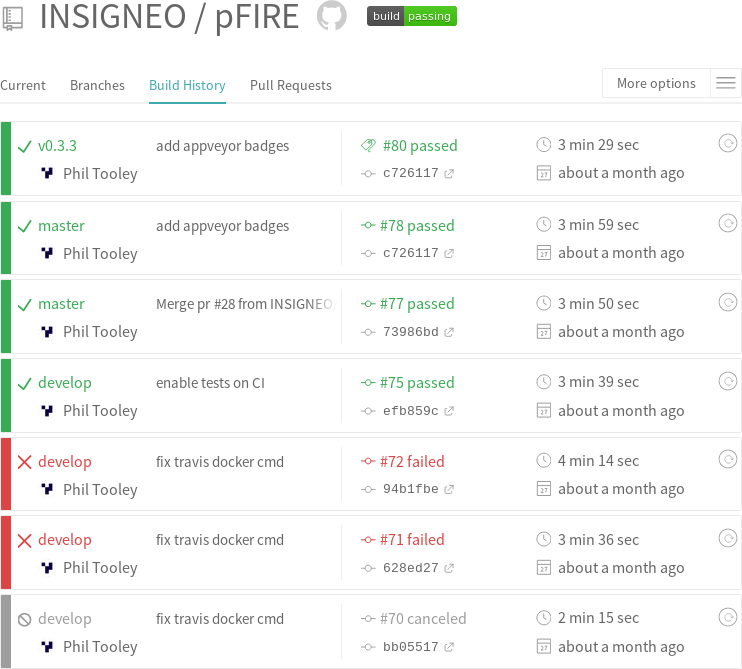
\includegraphics[width=\textwidth]{travis}
  \end{columns}
\end{frame}

\begin{frame}
  \frametitle{Conclusions}
  \begin{block}{Writing high quality HPC code is not easy, but...}
    \begin{itemize}
      \item Lots of options for applying HPC to a problem
        \begin{itemize}
          \item[] determine appropriate approach based on current and future needs
        \end{itemize}
      \item Using high-level frameworks provides all the building blocks
        \begin{itemize}
          \item[] e.g PETSc for parallel linear algebra, Spark for big data
        \end{itemize}
      \item Small changes can bring big gains
        \begin{itemize}
          \item[] parallelising just the slowest part can really help with speed 
        \end{itemize}
      \item Software development best practice helps create robust software
        \begin{itemize}
          \item[] regular testing finds bugs early, version control makes fixing them easier
        \end{itemize}
    \end{itemize}
  \end{block}
  \begin{block}{With the right tools, \emph{anyone} can write good HPC code}
  \end{block}
  \vspace{0.5em}
\end{frame}

\begin{frame}
  \centering
  
\includegraphics[width=0.4\textwidth]{cute_toothless}
  \begin{center}
    Thank You
  \end{center}
\end{frame}

\begin{frame}
  \frametitle{Useful Resources}
  \begin{itemize}
    \item\alert{Slides:} https://github.com/ptooley/hpc\_dragons
    \vspace{0.3em}
    \item\alert{RSE Code Clinic:}
    \begin{itemize}
      \item[] \alert{Free 30 minute advice sessions:} https://rse.shef.ac.uk/support/code-clinic/
    \end{itemize}
    \vspace{0.3em}
    \item\alert{Best Practice Guidance}
    \begin{itemize}
      \item[]\alert{RSE@Sheffield:} https://rse.shef.ac.uk
      \item[]\alert{SSI:} https://software.ac.uk
    \end{itemize}
    \vspace{0.3em}
    \item\alert{HPC Programming}
    \begin{itemize}
      \item[]\alert{PRACE Training:} http://www.training.prace-ri.eu/ 
      \item[]\alert{LLNL Online Training:} https://hpc.llnl.gov/training/tutorials
      \item[]\alert{GPU@Sheffield:} http://gpucomputing.shef.ac.uk/
      \item[]\alert{ShARC Documentation:} http://docs.hpc.shef.ac.uk/en/latest/sharc/
    \end{itemize}
  \end{itemize}
  \vspace{0.3em}
\end{frame}

\begin{frame}[plain]
  \centering
  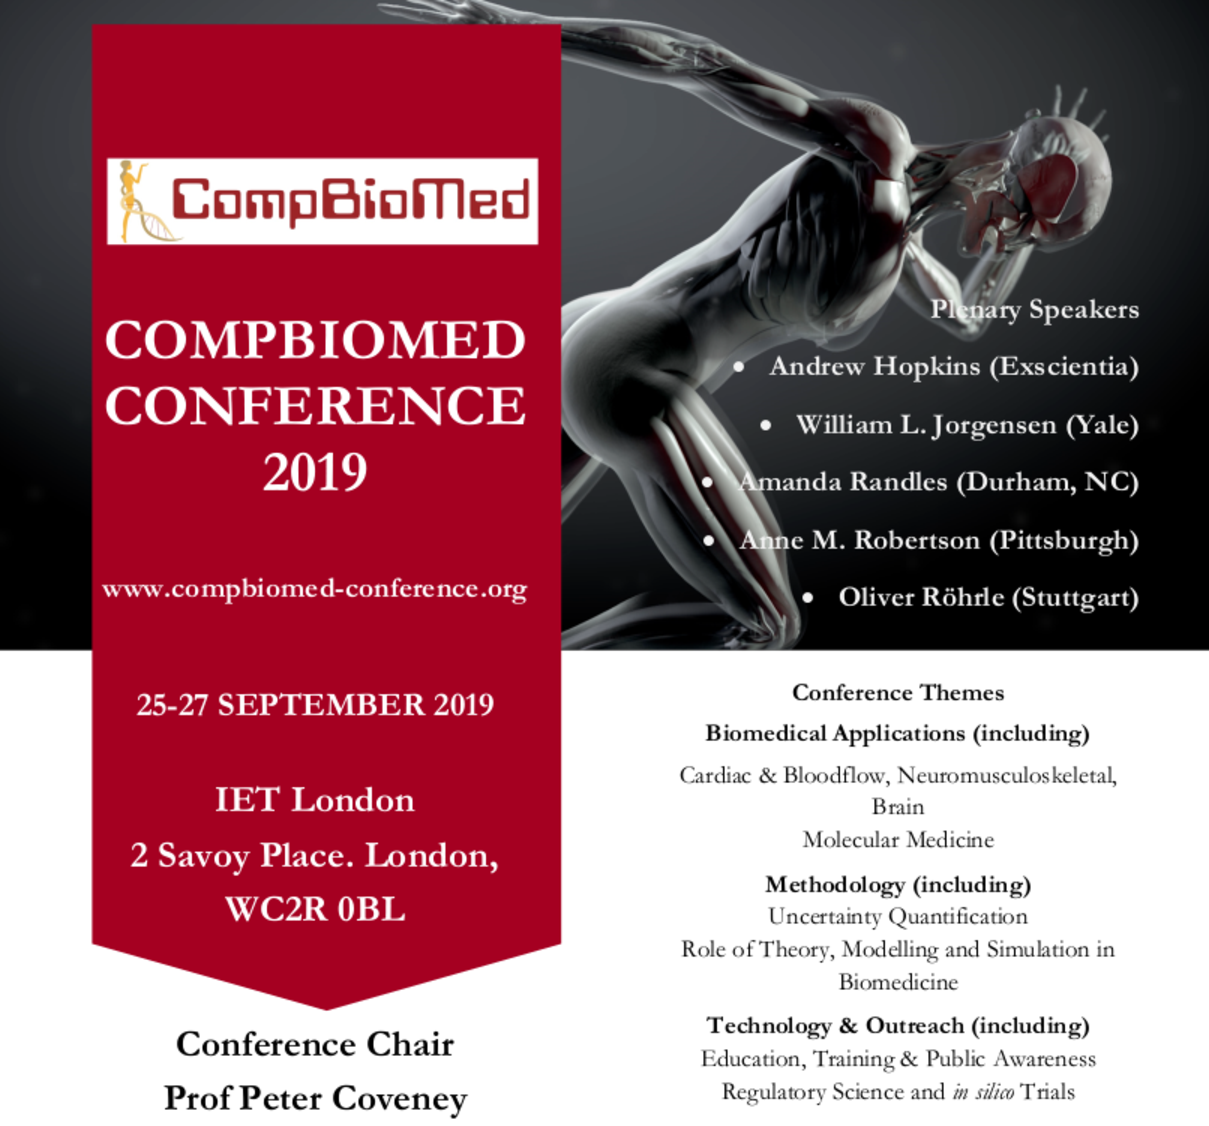
\includegraphics[height=\textheight]{cbmcflier}
\end{frame}

\end{document}

